\documentclass[17pt]{article}

\usepackage[margin=1in, paperwidth=8.5in, paperheight=11in]{geometry}
\usepackage{amsmath}
\usepackage[document]{ragged2e}
\usepackage{graphicx}
\usepackage{listings}
\usepackage{color}
\usepackage[none]{hyphenat}

\begin{document}

\title{{Exercise 2}}
\author{Dejan Porjazovski}
\maketitle

\section{Question 1}

\subsection{The recognition result is very sensitive to the vocabulary of the evaluation data and the lexicon used for recognition. To improve the recognition accuracy, a second lexicon material/ex2/w150.dict is provided which contains only those words that appear in the evaluation set. Build a recognition network from that and run the recognition test over the evaluation set. Compare the results to those of the larger lexicon. Why is the accuracy improving?}

With the w600.dict we got error of 36.84, compared to 15.44 when we used the w150.dict \\~\

The second lexicon 'w150.dict' contains only the words that appear in the
evaluation set so, when we try to predict the evaluation set, the model has already seen those words and that is why it predicts them better than the other dictionary where it has a lot more words. 

\subsection{The recognition network should reflect the recognition task. The task in this exercise contains only single words, but the recognition network contains a loop which allows multiple words to be recognized from a single utterance. Remove the loop by modifying the recognition network (built from w150.dict) with a text editor. Run the recognition test once more and compare to previous results. Explain why the accuracy changed.}

The loop allows multiple words to be recognized from a single utterance,
which means that the recognized word will have additional words after it.
By removing the loop, we eliminated those additional words and improved the accuracy.


\section{Question 2}

\subsection{An easy way of tracking the HMM training process is to look at the logarithmic likelihood values reported by HERest. You can fetch them with the command grep "average log prob" hmm-?/train*log. Plot the values as one continuous line. (Check that grep gave them in the right order!)}

\begin{center}
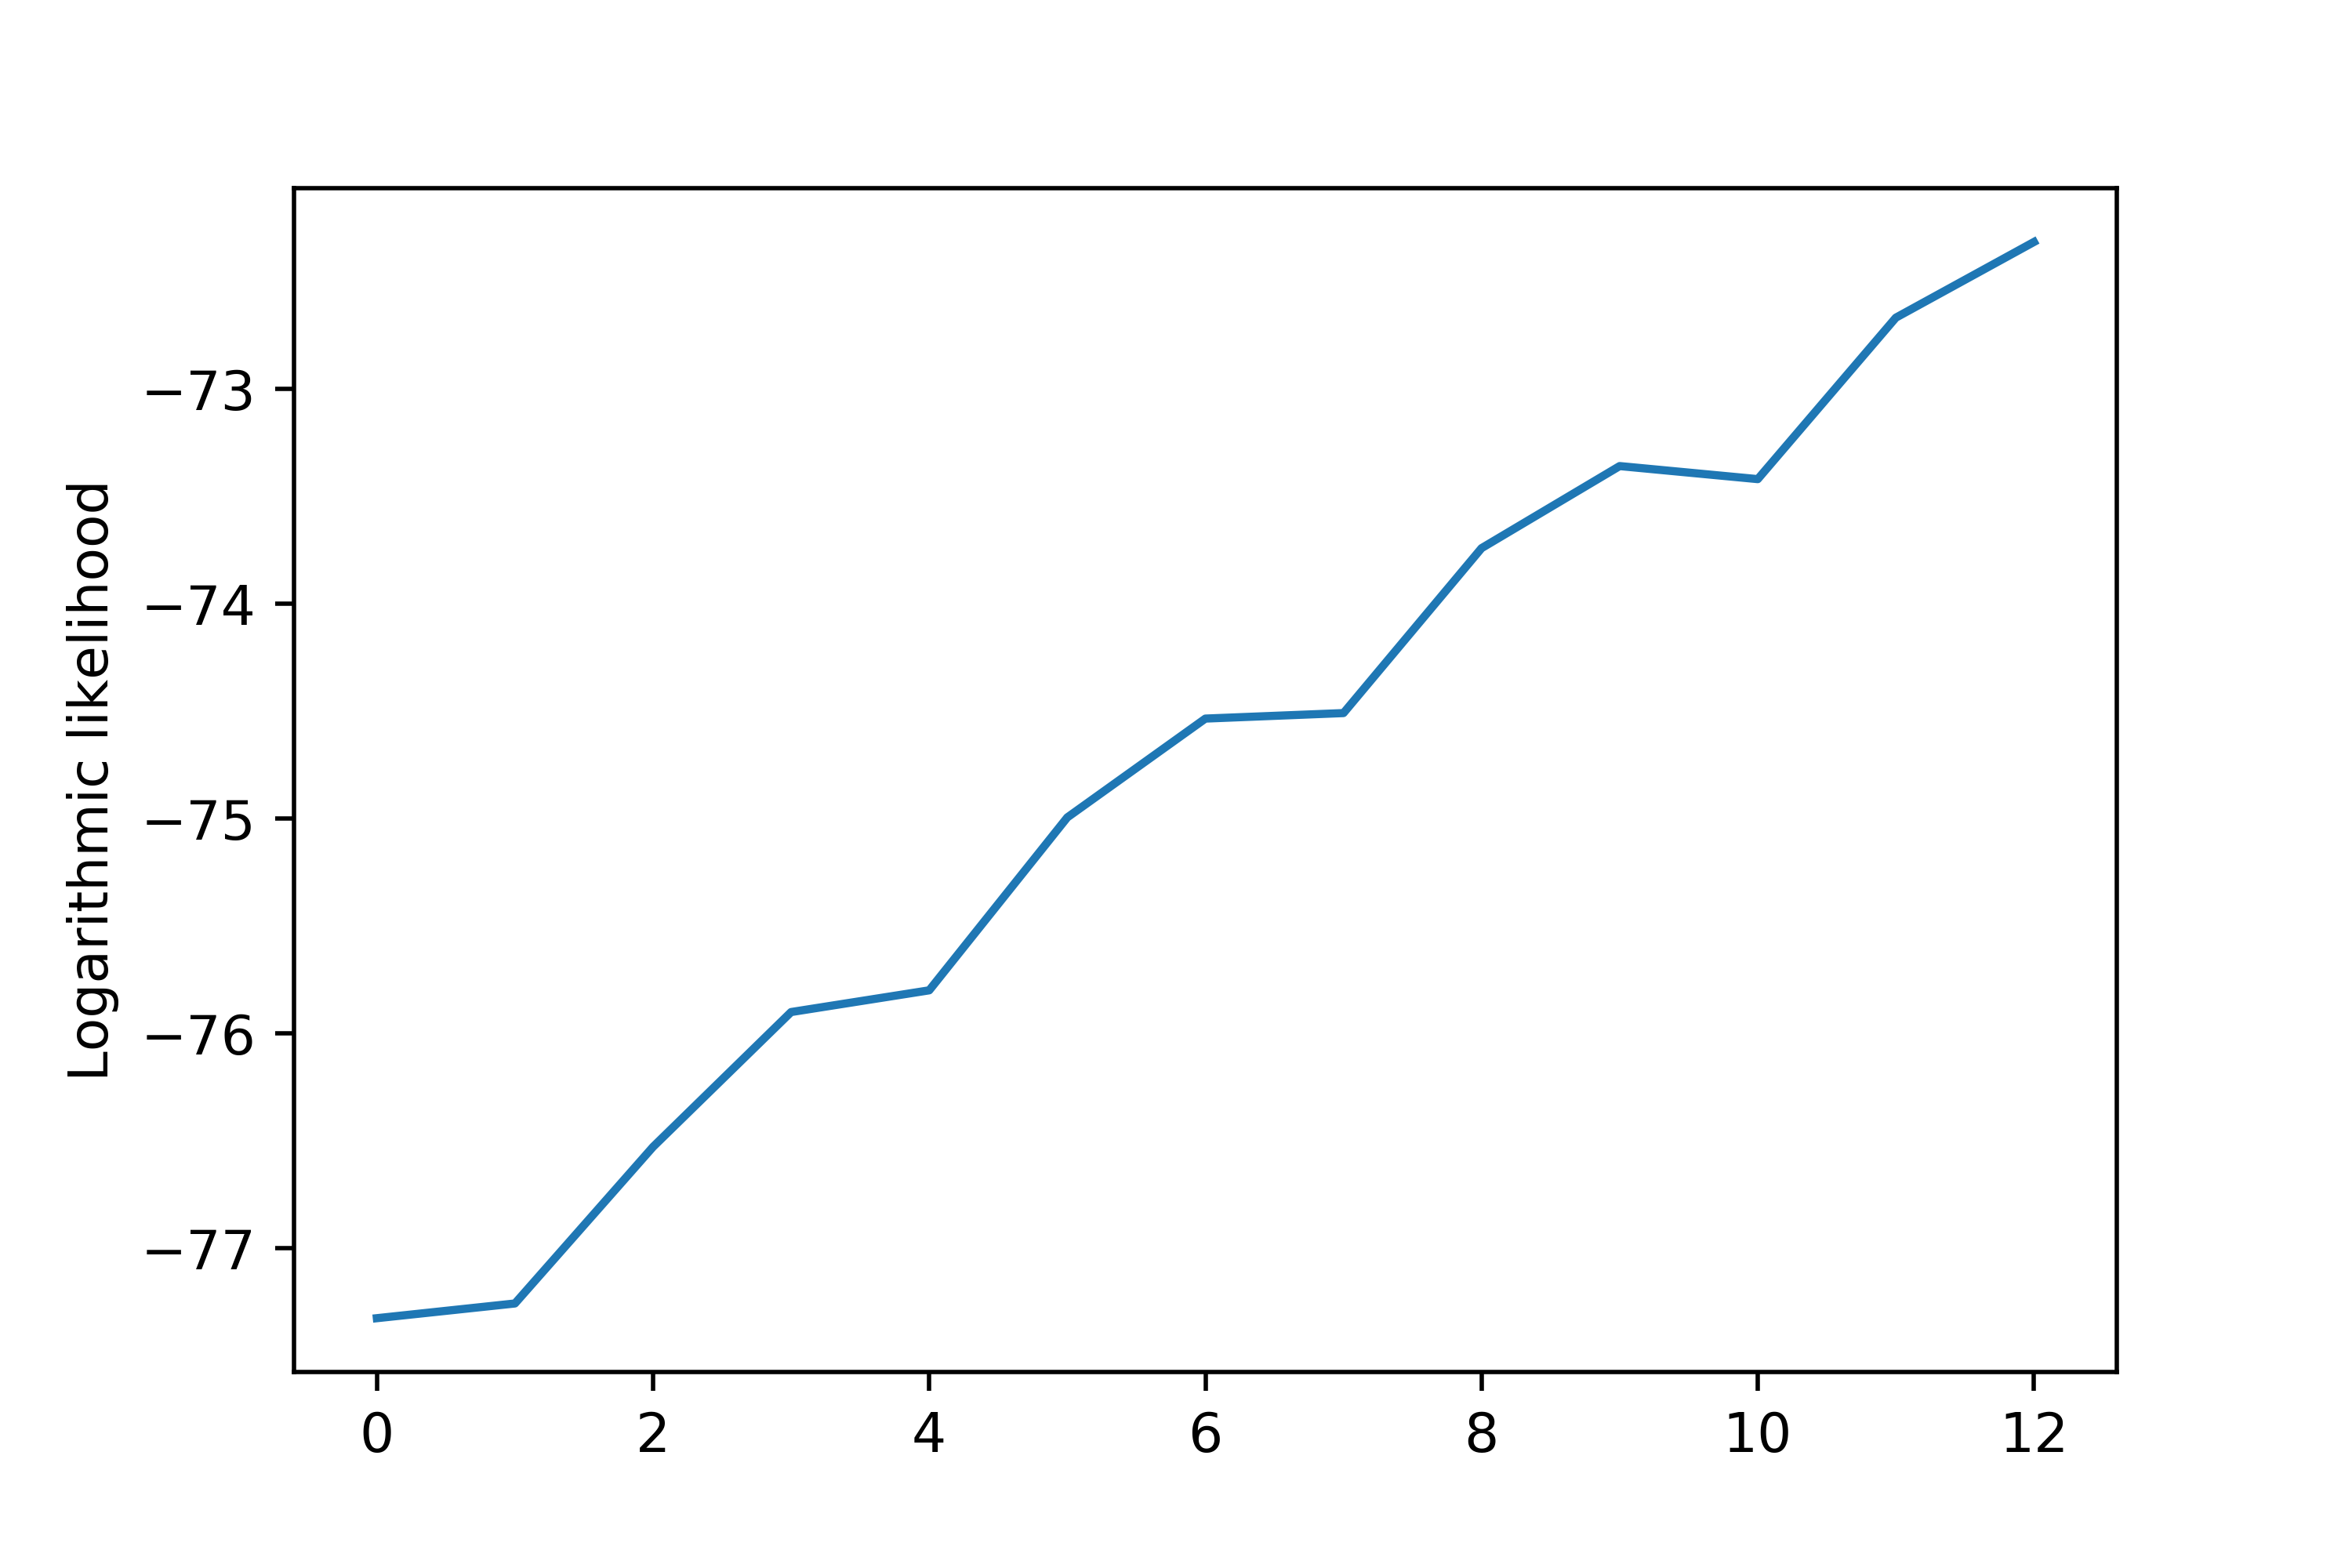
\includegraphics[width=15cm, height=8cm]{likelihood.png}
\end{center}

\subsection{Using the modified w150 network, recognize the evaluation set using all the models through hmm-2 to hmm-6. Graphically plot the word error rate with respect to the model number. Comment on the relationship of the two curves. Do you think further iterations would improve the recognition result?}

\begin{center}
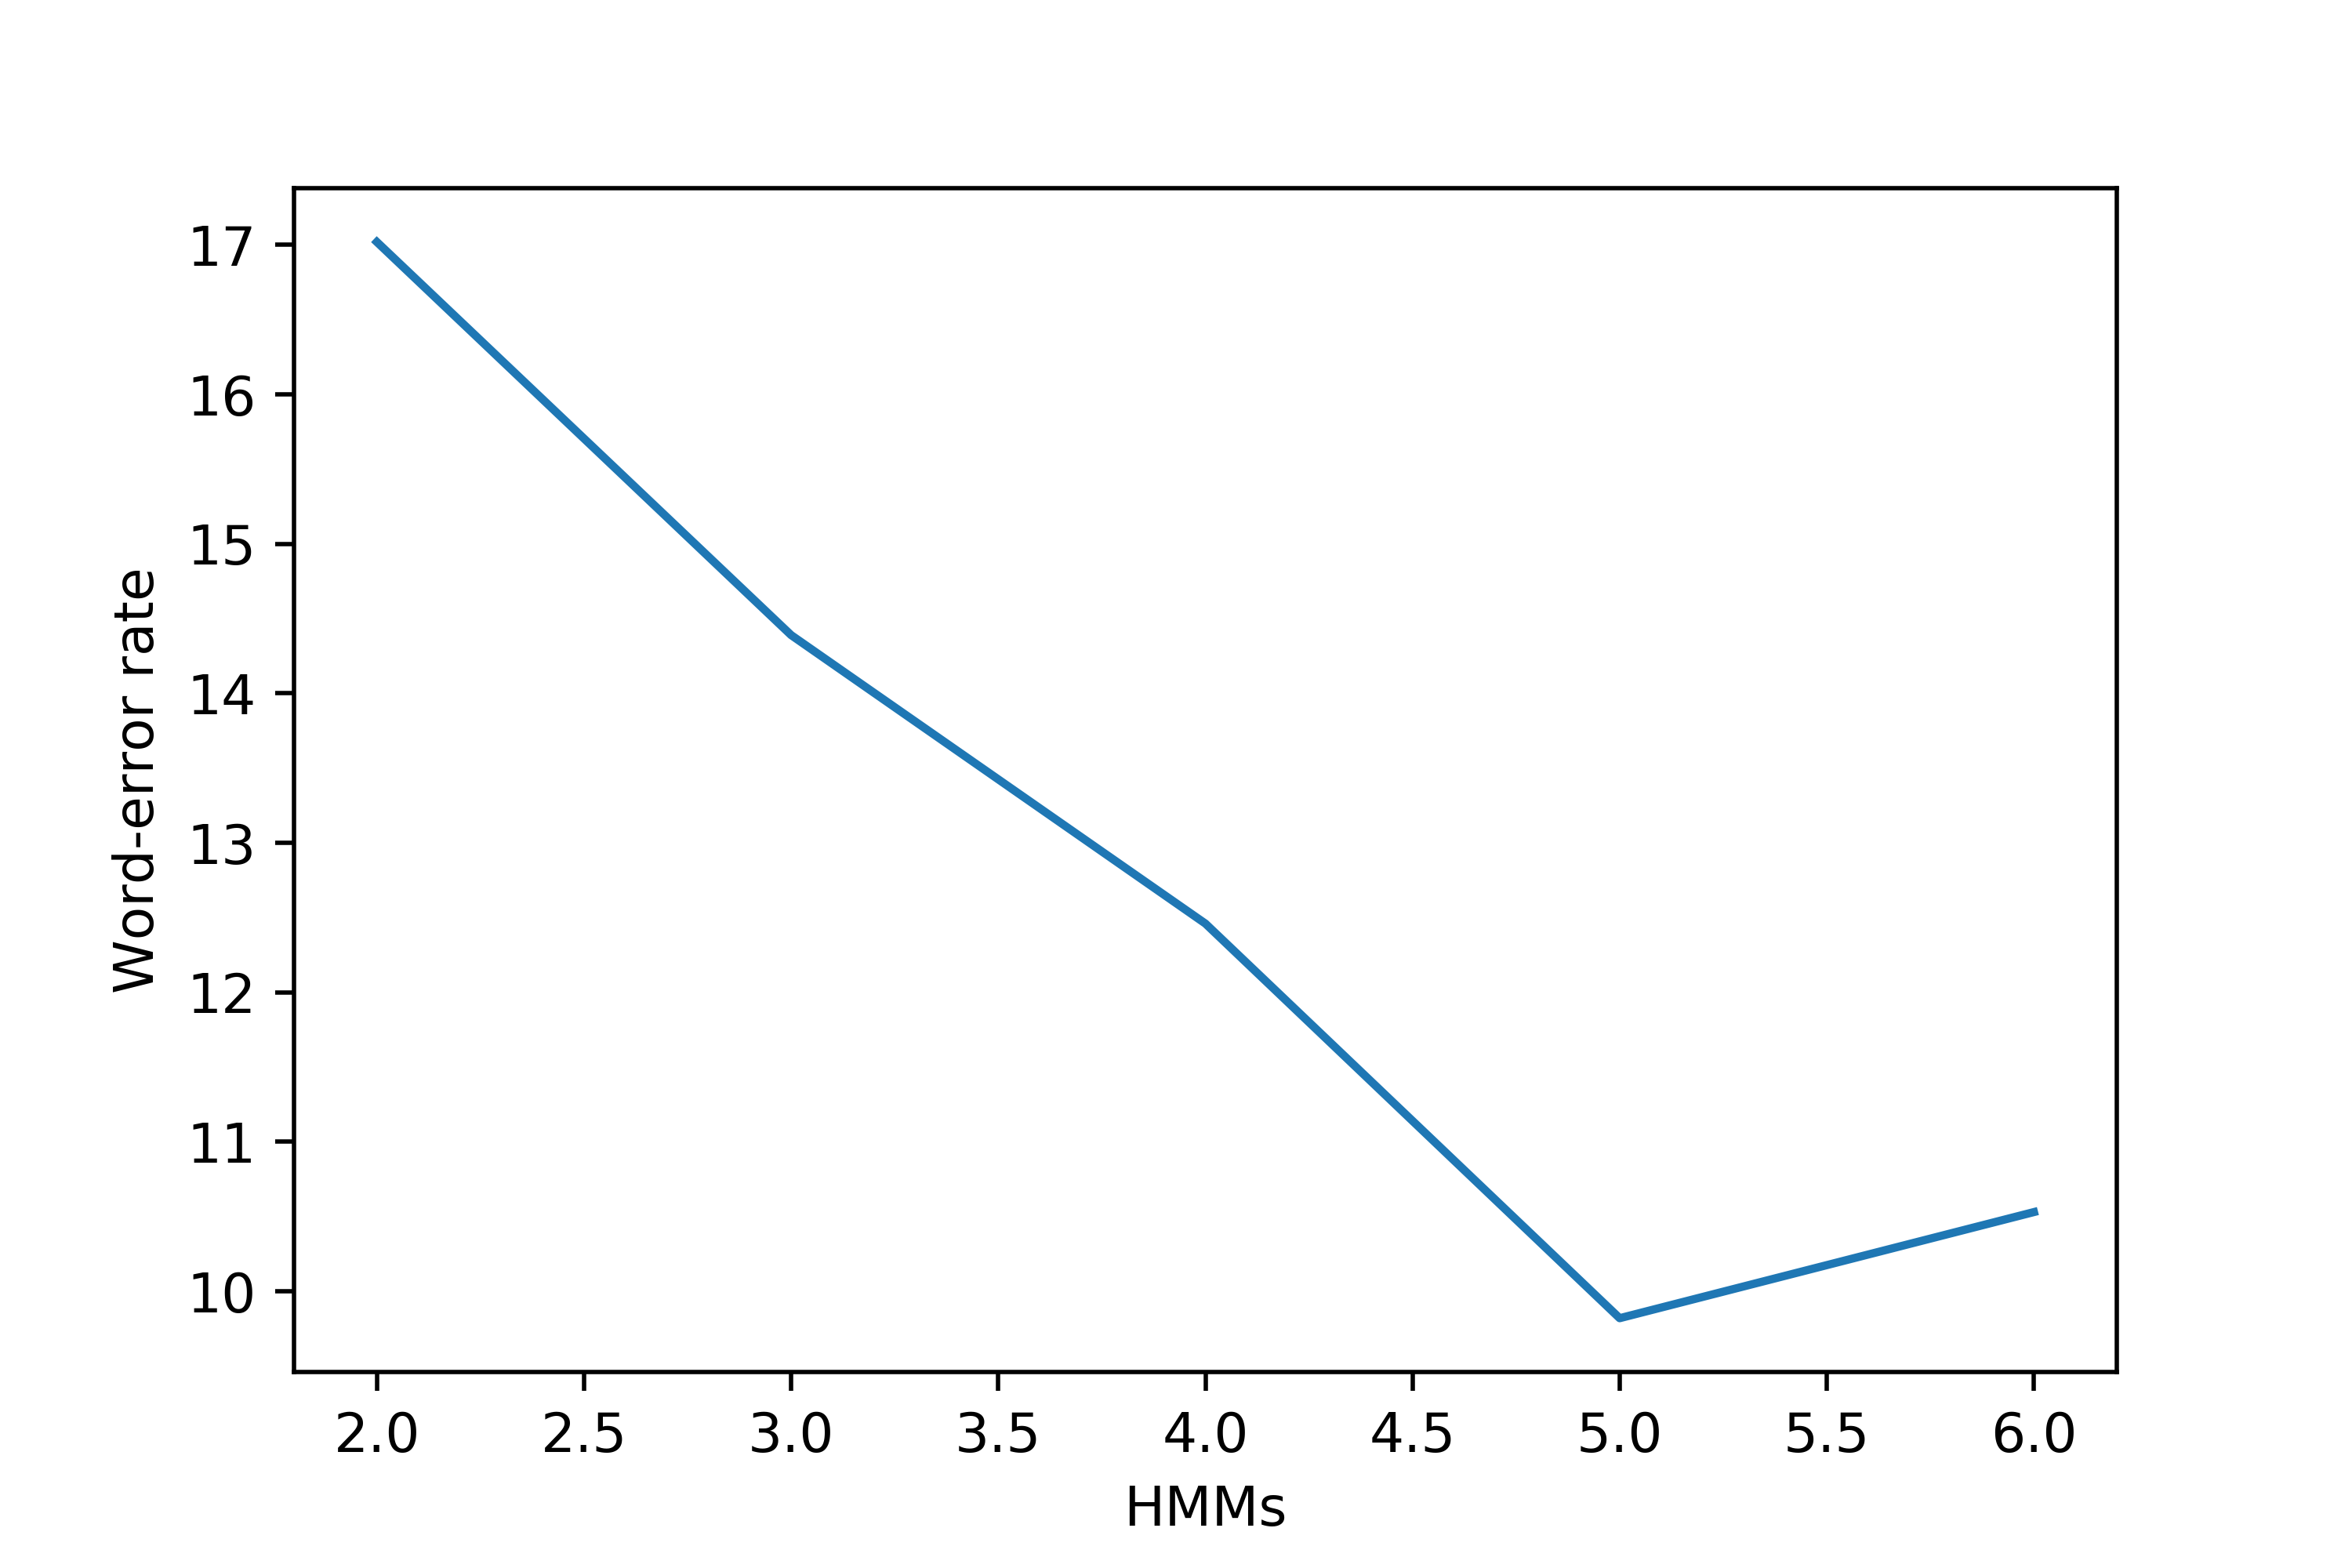
\includegraphics[width=15cm, height=8cm]{word_error_rate.png}
\end{center}

From the two curves we can see that when we increase the number of HMMs, both the log probability and the word-error rate decrease. \\
For the word-error rate, if we use more than 5 HMMs, the error starts increasing. \\~\\

Further iterations would not improve the recognition results for the word-error rate because from the curve we can see that until hmm - 5, the error drops but on hmm - 6 it increases. So, if we use more iterations, the recognition result will probably not improve.


\section{Question 3}

\subsection{Recognize the evaluation set with the gender dependent models, using correct evaluation subsets f for females and m for males. Use the modified w150 network. Report the individual recognition performances of the subsets as well as the combined one. Compare the results to the subset and combined results of the gender independent model. Given the subset result files, you can get the combined results with HResult simply by providing both input files at the same time.}

The word-error rate for the female subset is 12.22 \\
The word-error rate for the male subset is 7.00 \\
The combined word-error rate is 9.47 \\

\subsection{Test what would happen if you accidentally used the female model to recognize male set and vice versa. Report the combined recognition result for this case. Comment the possible benefits and drawbacks of gender dependent models.}

When I used male model with female set, I got word-error rate of 23.79 \\
When I used female model with male set, I got word-error rate of 31.00 \\
The combined word-error rate for the mixed models is 27.59 \\~\\

Most parametric representations of speech are highly speaker dependent and probability distributions suitable for one gender may not perform as well for the other gender. \\~\\
If we have gender dependent models, we should be able to predict speech more accurately because there are differences in male and female speech. \\
For example, female speakers tend to have higher pitch. \\~\\
A drawback for this approach is that we need to have more data since we are having separate models for the genders. \\~\\


\subsection{Report the number of Gaussians in the final models. For a model under hmm-6, you can fetch it with command}

Number of gaussians for males:
\begin{itemize}
	\item{hmm-6 = 757}
	\item{hmm-5 = 533}
	\item{hmm-4 = 383}
	\item{hmm-3 = 262}
	\item{hmm-2 = 133}
\end{itemize}


Number of gaussians for females:
\begin{itemize}
	\item{hmm-6 = 304}
	\item{hmm-5 = 288}
	\item{hmm-4 = 265}
	\item{hmm-3 = 221}
	\item{hmm-2 = 133}
\end{itemize}


Number of gaussians for gender independent:
\begin{itemize}
	\item{hmm-6 = 1058}
	\item{hmm-5 = 658}
	\item{hmm-4 = 425}
	\item{hmm-3 = 266}
	\item{hmm-2 = 133}
\end{itemize}


\end{document}

















